\chapter{Dice Operation and UART}

\section{Dice Operation}

Lab 7 calls for a build version on GPIO channel~1 and debounced \texttt{BTNU}
and \texttt{SW[3:0]} on GPIO channel~2. A press of \texttt{BTNU} should
roll each selected die, update its digit, and send the result through UART.
The current snapshot contains a single-channel GPIO and the LED test firmware.

\todo{Document the GPIO wiring, version readback, dice generation, and UART output for the board build.}

\section{Running Setup}

Figure~\ref{fig:basys3-running} shows the dice application running on the
Digilent BASYS3. The project uses Vivado and Vitis 2025.2.

\begin{figure}[!htbp]
  \centering
  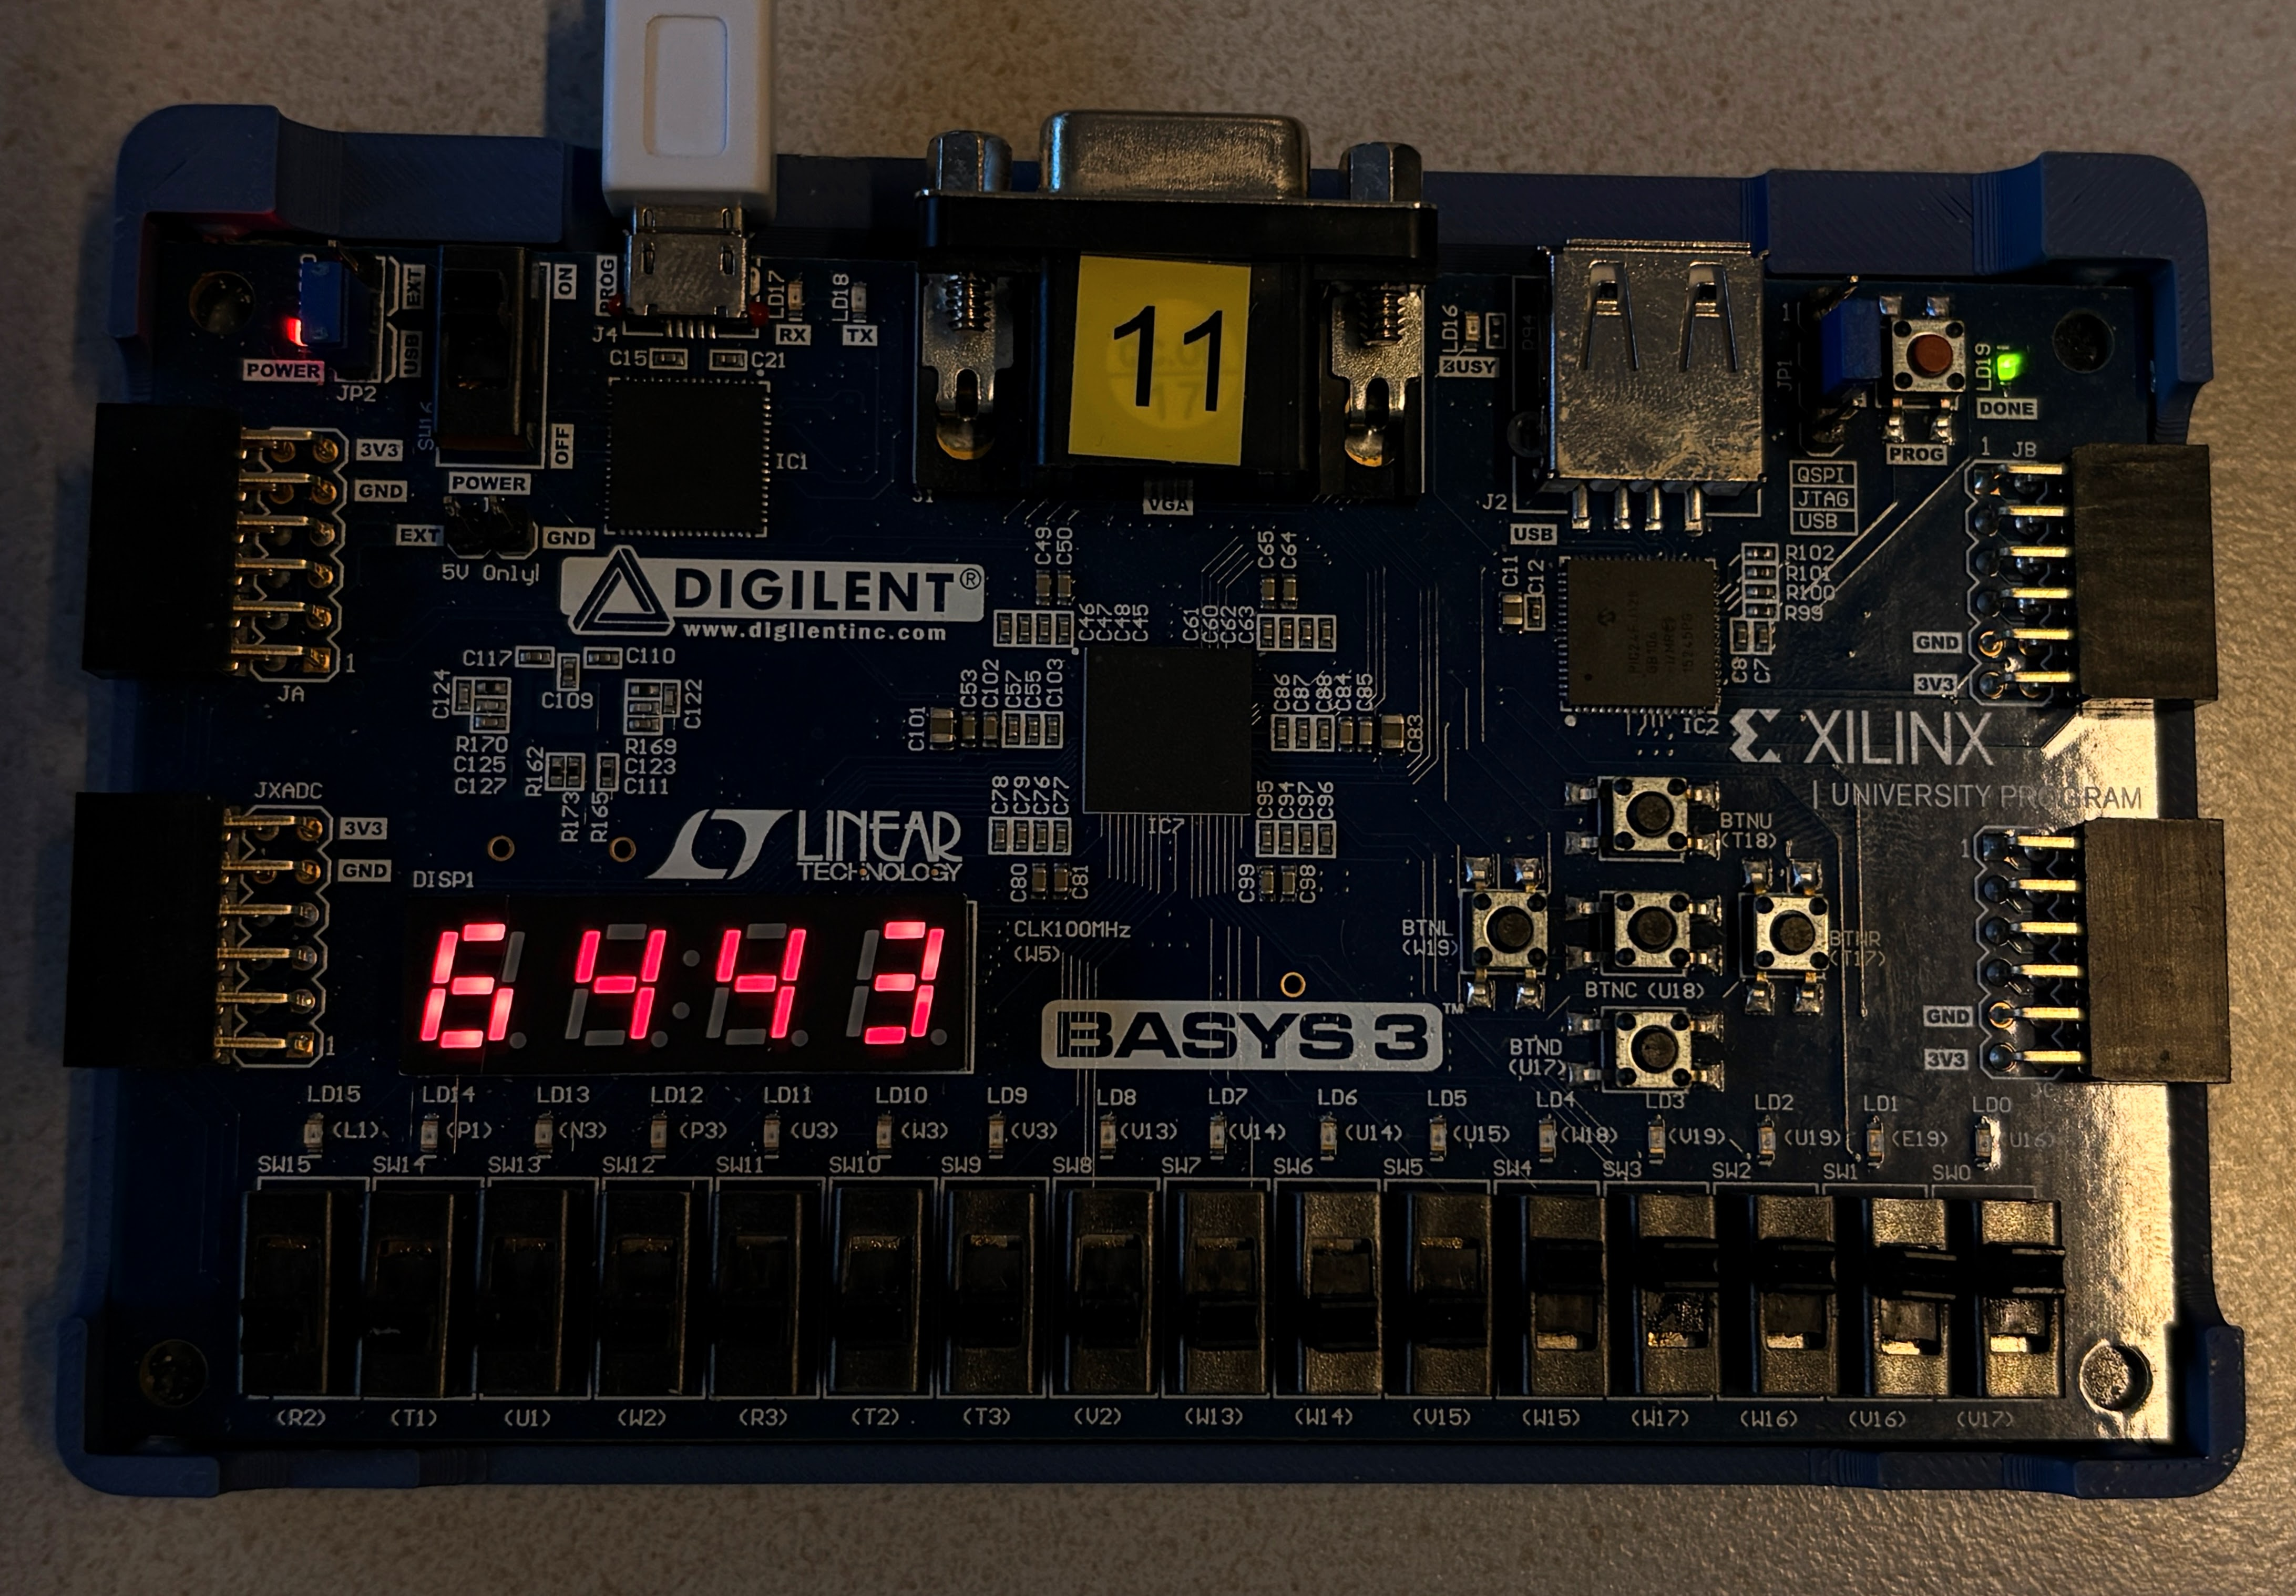
\includegraphics[width=\linewidth]{figures/final/basys3-running.jpg}
  \caption{BASYS3 board no. 11 displaying dice results 6, 4, 4, and 3.}
  \label{fig:basys3-running}
\end{figure}

\IfFileExists{figures/final/uart.png}{%
  \evidencefigure{uart.png}{Serial terminal showing dice results from the running board.}{fig:uart}{}%
}{}
